\documentclass[tikz]{standalone}
\usepackage{tikz,amsmath}
\usetikzlibrary{shapes}
\begin{document}
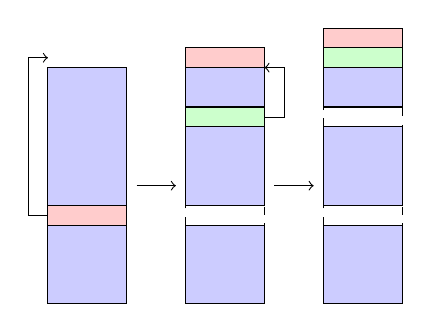
\begin{tikzpicture}
    \draw [fill = blue!20] (6.75,0) -- (6.75,3) -- (7.75,3) -- (7.75,0) -- cycle;
    \draw [fill = red!20] (6.75,1) -- (6.75,1.25) -- (7.75,1.25) -- (7.75,1) -- cycle;
    \draw [->] (6.75,1.125) -- (6.5,1.125) -- (6.5,3.125) -- (6.75,3.125);

    \draw [->] (7.875,1.5) -- (8.375,1.5);

    %\draw [dashed] (8.75,0) -- (8.75,3) -- (9.75,3) -- (9.75,0) -- cycle;
    \draw [fill = blue!20] (8.5,0) -- (8.5,1) -- (9.5,1) -- (9.5,0) -- cycle;
    \draw [dashed] (8.5,1) -- (8.5,1.25) -- (9.5,1.25) -- (9.5,1) -- cycle;
    \draw [fill = blue!20] (8.5,1.25) -- (8.5,3) -- (9.5,3) -- (9.5,1.25) -- cycle;
    \draw [fill=red!20] (8.5,3.25) -- (8.5,3) -- (9.5,3) -- (9.5,3.25) -- cycle;
    \draw [fill=green!20] (8.5,2.25) -- (8.5,2.5) -- (9.5,2.5) -- (9.5,2.25) -- cycle;
    \draw [->] (9.5,2.365) -- (9.75,2.365) -- (9.75,3) -- (9.5,3);

    \draw [->] (9.625,1.5) -- (10.125,1.5);

    \draw [fill = blue!20] (10.25,0) -- (10.25,1) -- (11.25,1) -- (11.25,0) -- cycle;
    \draw [dashed] (10.25,1) -- (10.25,1.25) -- (11.25,1.25) -- (11.25,1) -- cycle;
    \draw [fill = blue!20] (10.25,2.5) -- (10.25,3) -- (11.25,3) -- (11.25,2.5) -- cycle;
    \draw [fill = blue!20] (10.25,2.25) -- (10.25,1.25) -- (11.25,1.25) -- (11.25,2.25) -- cycle;
    \draw [fill=green!20] (10.25,3.25) -- (10.25,3) -- (11.25,3) -- (11.25,3.25) -- cycle;
    \draw [fill=red!20] (10.25,3.5) -- (10.25,3.25) -- (11.25,3.25) -- (11.25,3.5) -- cycle;
    \draw [dashed] (10.25,2.25) -- (10.25,2.5) -- (11.25,2.5) -- (11.25,2.25) -- cycle;
\end{tikzpicture}
\end{document}
